% Appendix Template

\chapter{Registro de datos por participante} % Main appendix title

\label{App_Registro} % Change X to a consecutive letter; for referencing this appendix elsewhere, use \ref{AppendixX}

El experimento fue programado de manera que los datos obtenidos sobre la ejecución de cada participante fueran registraran en un archivo CSV, creado bajo un título que le asignara un número e indicara sus iniciales y la fecha y experimento en que participó.\\

La Figura~\ref{fig:csv} presenta parte de un CSV creado a partir de la ejecución de uno de los participantes del Experimento 2, (se muestran los primeros seis ensayos).\\

\begin{figure}[th]
\centering
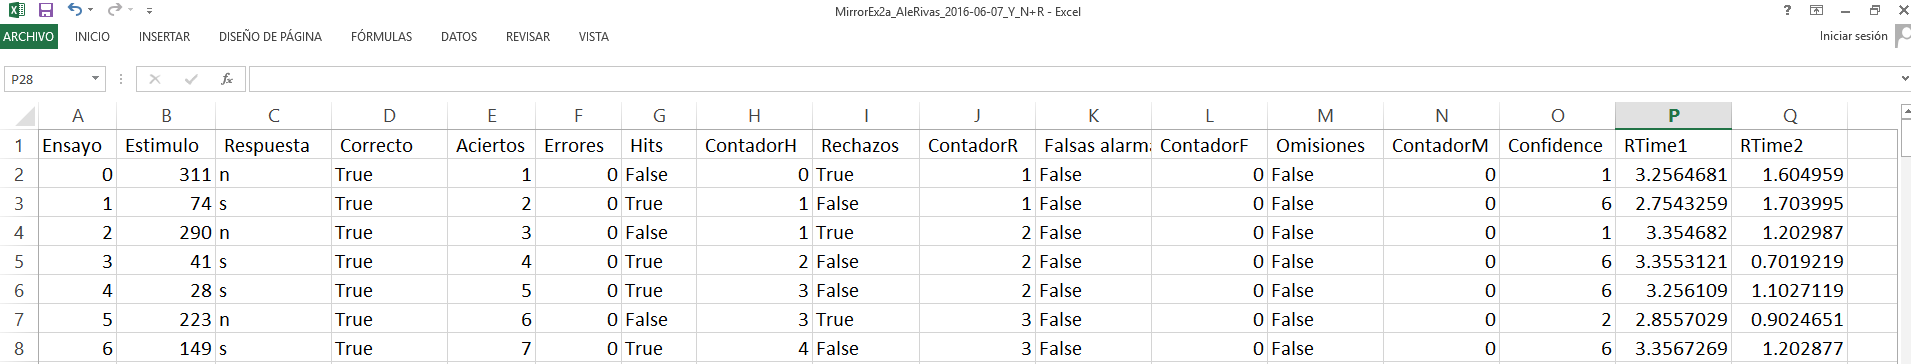
\includegraphics[width=0.95\textwidth]{Figures/csv} 
\decoRule
\caption[CSV muestra]{Captura de pantalla de uno de los archivos CSV generados tras la aplicación del experimento. Se ilustra el registro y clasificación de las respuestas emitidas por los participantes en cada ensayo, en función de su correspondencia con el estímulo aleatoriamente mostrado.}
\label{fig:csv}
\end{figure}
\end{itemize}

Por cada uno de los 640 ensayos realizados, el programa registró información acerca de: 1) cuál de los estímulos diseñados -ver~\ref{Cap_Exp}- fue presentado (\textit{Estímulo}); 2) qué respuesta emitió el participante (\textit{Respuesta}); 3) si ésta fue correcta o no (\textit{Correcto}); 4) el total de aciertos acumulados hasta entonces (\textit{Aciertos}); 5) el total de errores acumulados (\textit{Errores}); 6) qué tipo de resultado se obtuvo (\textit{Hits, Rechazos, Falsas alarmas, Omisiones}); 7) un contador con el número acumulado de cada resultado (\textit{ContadorH, ContadorF, ContadorR, ContadorM}); 7) el puntaje de confianza registrado de acuerdo con la Escala completa (\textit{Confidence}); 8) el tiempo de respuesta entre la presentación del estímulo y la emisión de una respuesta Sí/No (\textit{RTime1}) y 9) el tiempo de respuesta entre la aparición de la Escala de Confianza y la emisión de un puntaje (\textit{RTime2}).\\